%
% tikztemplate.tex -- template for standalon tikz images
%
% (c) 2019 Prof Dr Andreas Müller, Hochschule Rapperswil
%
\documentclass[tikz]{standalone}
\usepackage{amsmath}
\usepackage{times}
\usepackage{txfonts}
\usepackage{pgfplots}
\usepackage{csvsimple}
\usetikzlibrary{arrows,intersections,math}
\begin{document}
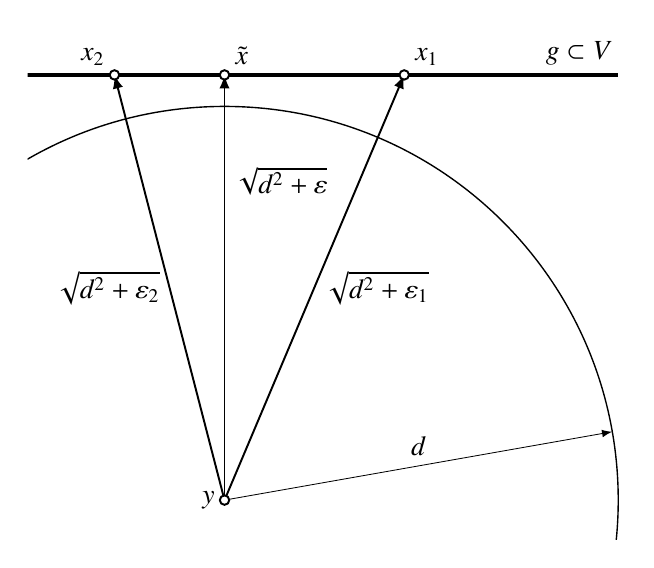
\begin{tikzpicture}[>=latex]

% add image content here

\begin{scope}
\clip (-2.5,-4.5) rectangle (5.1,2);

\def\d{1.4}

\draw[line width=1.4pt]  (-5,\d)--(5,\d);

\def\aone{25}
\def\atwo{-15}

\xdef\xone{({(4+\d)*sin(\aone)},\d)}
\xdef\xtwo{({(4+\d)*sin(\atwo)},\d)}
\def\xtilde{(0,\d)}

\draw[line width=0.5pt] (0,-4) circle[radius=5];

\def\punkt#1{
	\fill[color=white] #1 circle[radius=0.06];
	\draw[line width=0.7pt] #1 circle[radius=0.06];
}

\draw[->,line width=0.7pt] (0,-4)--\xone;
\draw[->,line width=0.7pt] (0,-4)--\xtwo;
\draw[->,line width=0.7pt] (0,-4)--\xtilde;

\draw[->,line width=0.3pt] (0,-4)--({5*cos(10)},{5*sin(10)-4});
\node at ({2.5*cos(10)},{2.5*sin(10)-4}) [above] {$d$};

\punkt{(0,-4)}
\punkt{\xone}
\punkt{\xtwo}
\punkt{\xtilde}

\node at \xtilde [above right] {$\tilde{x}$};
\node at \xone [above right] {$x_1$};
\node at \xtwo [above left] {$x_2$};

\node at (0,-4) [left] {$y$};

\node at ({(4+\d)*sin(\aone)/2},{0.5*(\d-4)}) [right] {$%\|y-x_1\|^2 =
\sqrt{d^2 + \varepsilon_1}$};
\node at ({(4+\d)*sin(\atwo)/2},{0.5*(\d-4)}) [left] {$%\|y-x_1\|^2 =
\sqrt{d^2 + \varepsilon_2}$};
\node at (0,{0.75*\d-1}) [right] {$\sqrt{d^2+\varepsilon}$};

\node at (4.5,\d) [above] {$g\subset V$};

\end{scope}

\end{tikzpicture}
\end{document}

